\section{Численные эксперименты незамкнутой цепи}
    Рассмотрим систему (\ref{flow}) при \(n=3\) со следующими коэффициентами:
    \begin{equation*}
        \begin{split}
            & \alpha_0 = 20, ~~ \alpha_1 = 16, ~~ \alpha_2 = 12, ~~ \alpha_3 = 8; \\
            & k_1 = 0.3, ~~ k_1 = 0.2, ~~ k_1 = 0.1; \\
            & m_1 = 4, ~~ m_1 = 3, ~~ m_1 = 2. \\ 
        \end{split}
    \end{equation*}
    Имеем трофические цепи длиной от \(q=1\) до \(q=3\). При заданных значениях параметров имеем данные интервалы, ограничивающие поступление внешнего ресурса \(Q\):
    \begin{enumerate}
        \item \(0 < Q < 12.5\);
        \item \(12.5 < Q < 95.83\dots\);
        \item \( 95.83\ldots < Q\).
    \end{enumerate}
    Варьируем значение \(Q\) и получаем графики численностей в равновесии.

    Для численного решения используем метод Рунге-Кутты \(4\)-порядка с шагом \(h = 0.01\). Начальные значения численностей равно \(2\). 
    
    Обозначения: <<Равн\(\{i\}\)>> -- значение точки равновесия, которой соответствует <<Вид\(\{i\}\)>>.

    \begin{figure}[H]
        \centering
        \begin{subfigure}[t]{.45\linewidth}
            \centering
            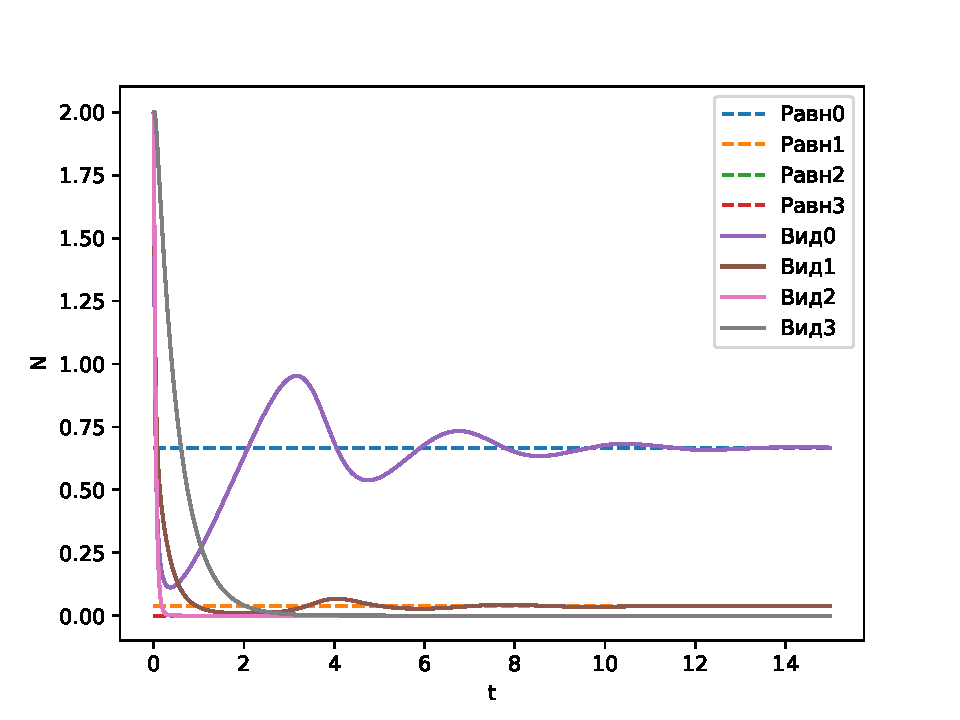
\includegraphics[width=\textwidth]{pictures/exp_flow/exp1_Q05.pdf}
            \caption{\(Q = 0.5\)}
        \end{subfigure}
        \begin{subfigure}[t]{.45\linewidth}
              \centering
              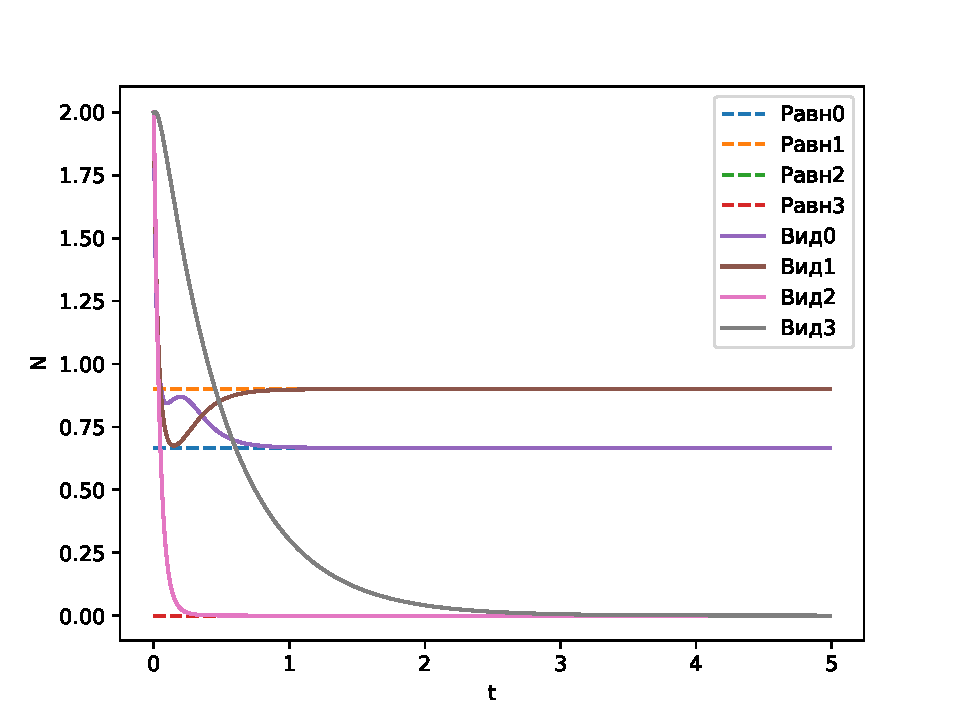
\includegraphics[width=\textwidth]{pictures/exp_flow/exp1_Q12.pdf}
              \caption{\(Q = 12\)}
            \end{subfigure}
        \caption{Численности видов системы, при \(Q\) близко к концам первого интервала.}  \label{fig:flow_exp1_q1}
    \end{figure}
    

    \begin{figure}[H]
        \centering
        \begin{subfigure}[t]{.45\linewidth}
            \centering
            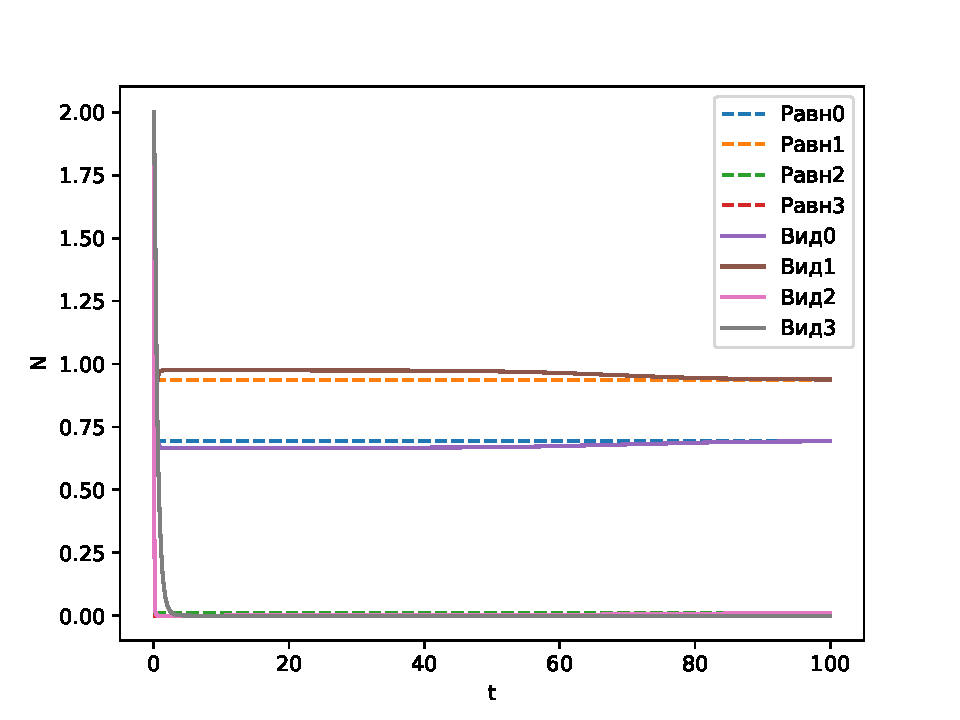
\includegraphics[width=\textwidth]{pictures/exp_flow/exp1_Q13.pdf}
            \caption{\(Q = 13\)}
        \end{subfigure}
        \begin{subfigure}[t]{.45\linewidth}
              \centering
              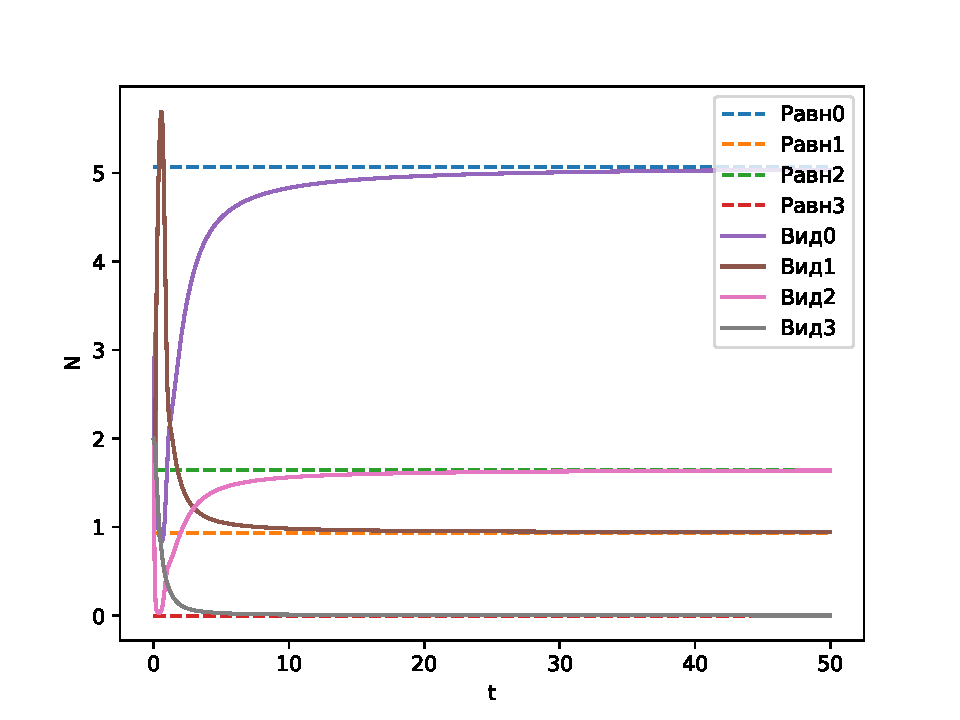
\includegraphics[width=\textwidth]{pictures/exp_flow/exp1_Q95.pdf}
              \caption{\(Q = 95\)}
            \end{subfigure}
        \caption{Численности видов системы, при \(Q\) близко к концам второго интервала.}  \label{fig:flow_exp1_q2}
    \end{figure}
    
    
    \begin{figure}[H]
        \centering
        \begin{subfigure}[t]{.45\linewidth}
            \centering
            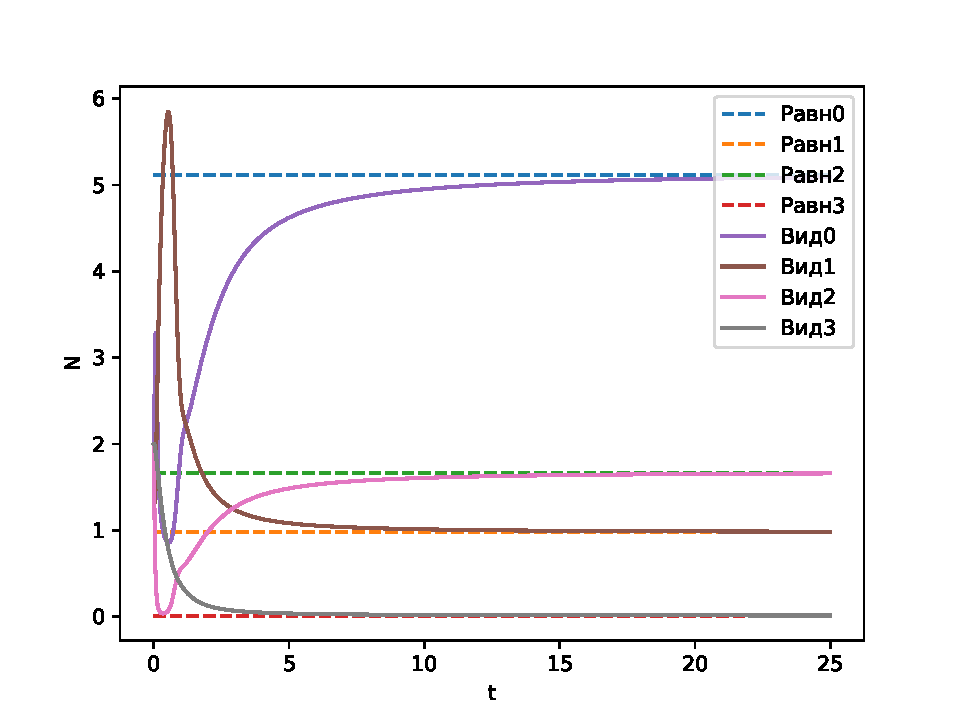
\includegraphics[width=\textwidth]{pictures/exp_flow/exp1_Q100.pdf}
            \caption{\(Q = 100, \quad N_3 \approx 0.0108\ldots \)}
        \end{subfigure}
        \begin{subfigure}[t]{.45\linewidth}
              \centering
              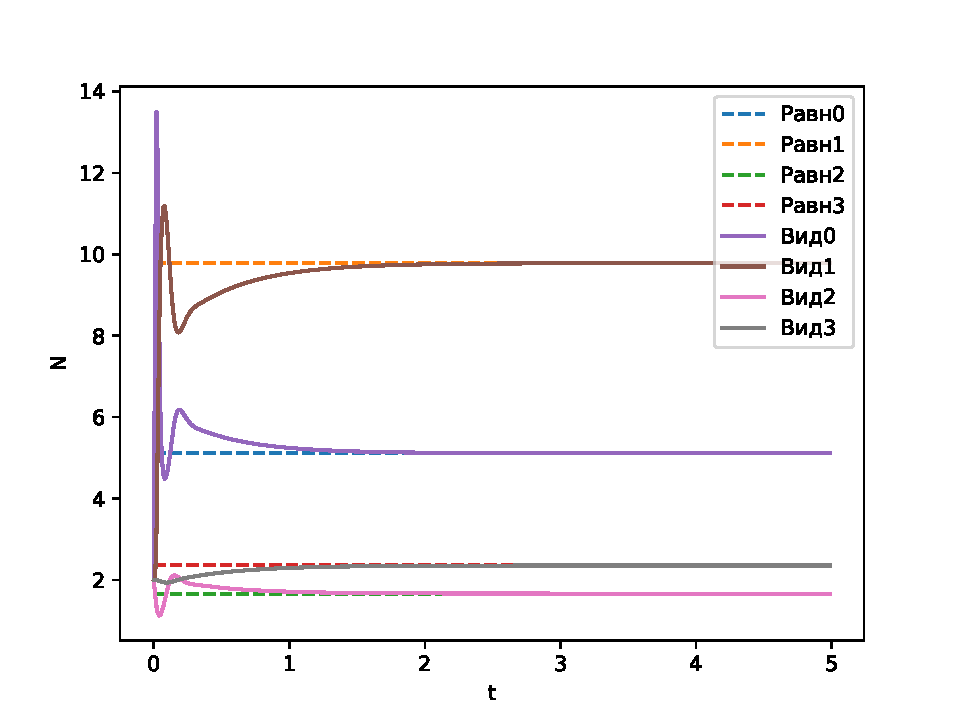
\includegraphics[width=\textwidth]{pictures/exp_flow/exp1_Q1000.pdf}
              \caption{\(Q = 1000\)}
            \end{subfigure}
        \caption{Численности видов системы, при \(Q\) близко к началу третьего интервала и на некотором отдалении.}  \label{fig:flow_exp1_q3}
    \end{figure}


    Для сравнения поведения системы при <<напряжённых>> трофических связях, возьмём систему (\ref{flow_full}) при трофических функциях \( V_i(x) = \alpha_i \arctan x  \). Т.е. виды могут насыщаться и не все его жертвы будут становиться добычей.
    

    \begin{figure}[H]
        \centering
        \begin{subfigure}[t]{.3\linewidth}
            \centering
            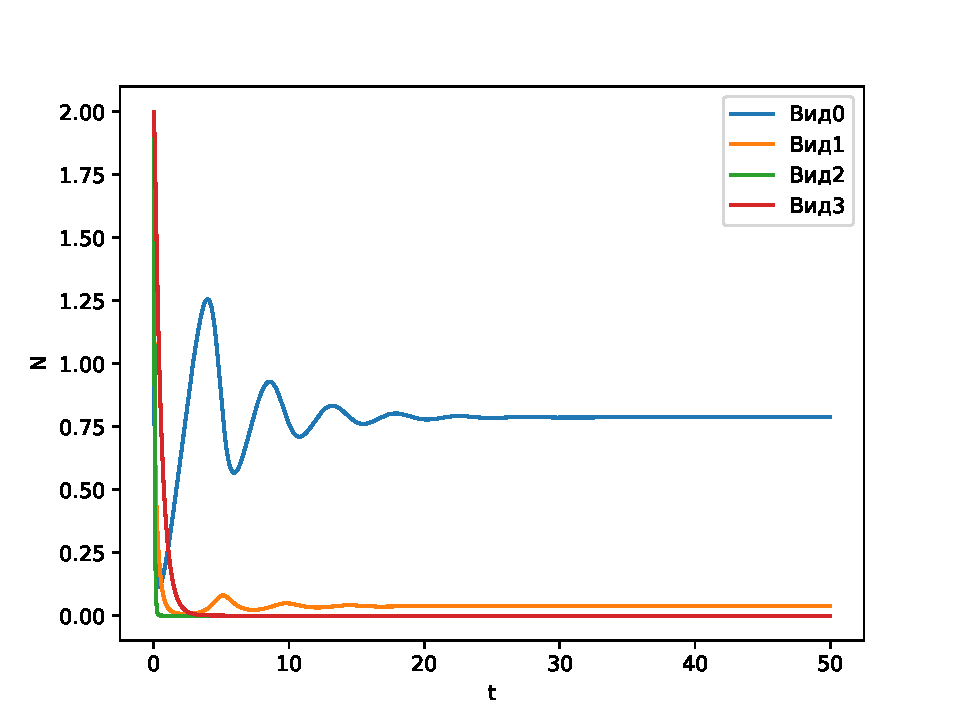
\includegraphics[width=\textwidth]{pictures/exp_flow/exp2_Q05.pdf}
            \caption{\(Q = 0.5\)}
        \end{subfigure}
        \begin{subfigure}[t]{.3\linewidth}
            \centering
            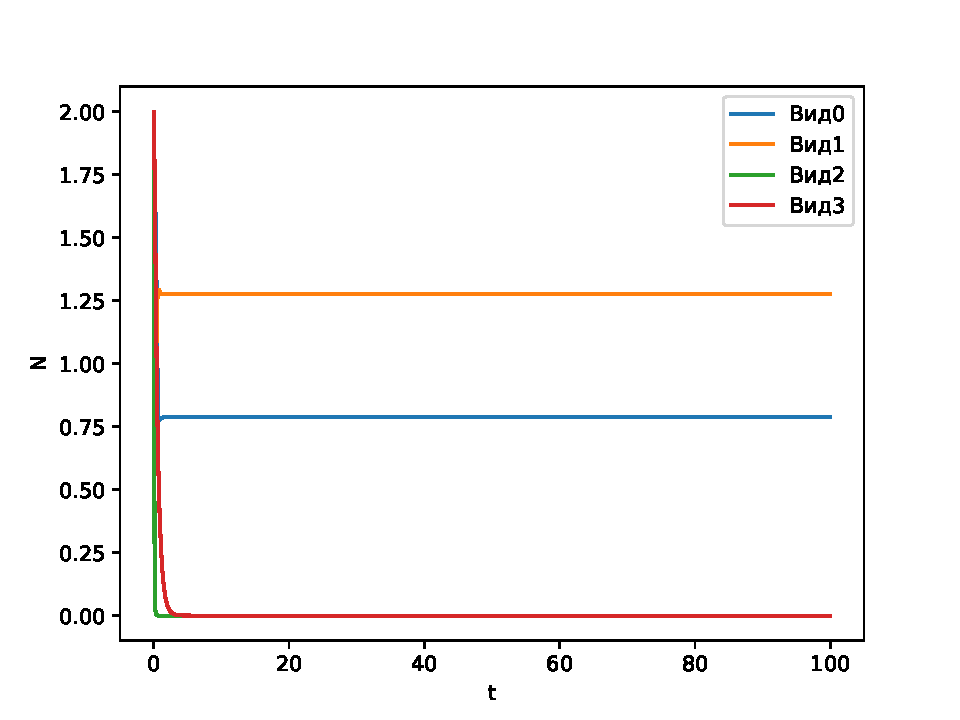
\includegraphics[width=\textwidth]{pictures/exp_flow/exp2_Q17.pdf}
            \caption{\(Q = 17\)}
        \end{subfigure}
        \begin{subfigure}[t]{.3\linewidth}
            \centering
            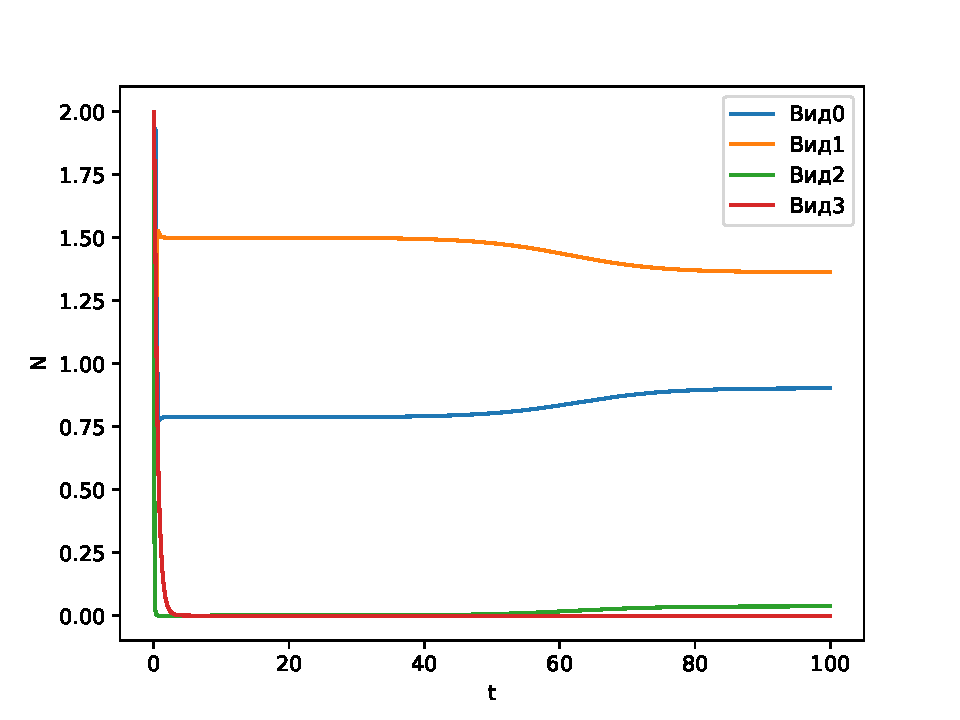
\includegraphics[width=\textwidth]{pictures/exp_flow/exp2_Q20.pdf}
            \caption{\(Q = 20\)}
        \end{subfigure}
        \caption{Численности видов системы.}  \label{fig:flow_exp2_q1}
    \end{figure}

    \begin{figure}[H]
        \centering
        \begin{subfigure}[t]{.3\linewidth}
            \centering
            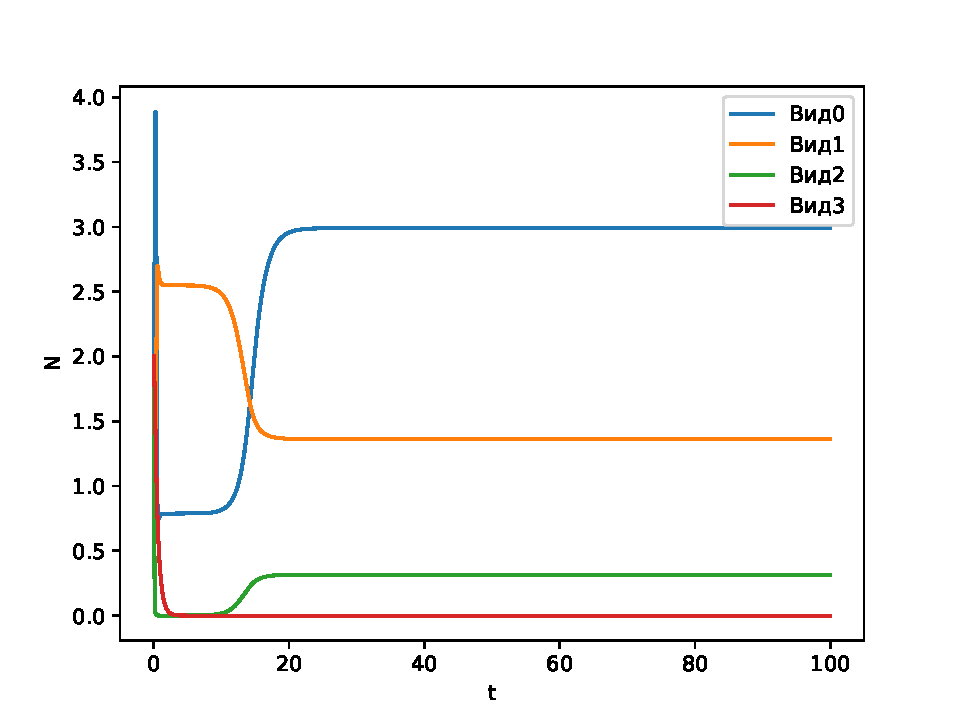
\includegraphics[width=\textwidth]{pictures/exp_flow/exp2_Q34.pdf}
            \caption{\(Q = 34\)}
        \end{subfigure}
        \begin{subfigure}[t]{.3\linewidth}
            \centering
            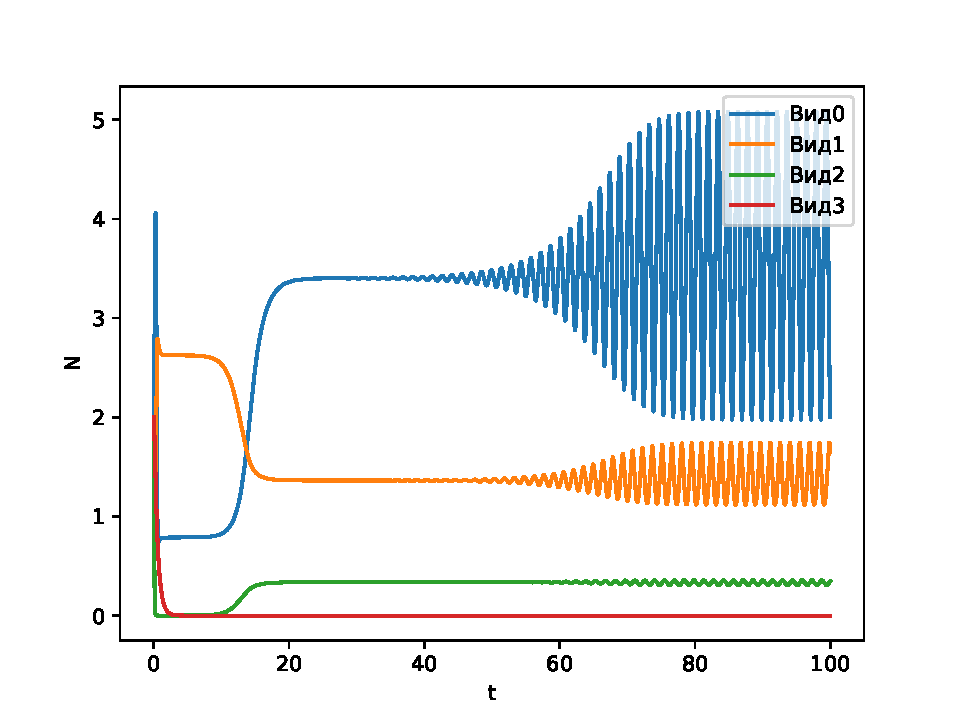
\includegraphics[width=\textwidth]{pictures/exp_flow/exp2_Q35.pdf}
            \caption{\(Q = 35\)}
        \end{subfigure}
    \caption{Численности видов системы.}  \label{fig:flow_exp2_q2}
    \end{figure}
    
    \begin{figure}[H]
        \centering
        \begin{subfigure}[t]{.3\linewidth}
            \centering
            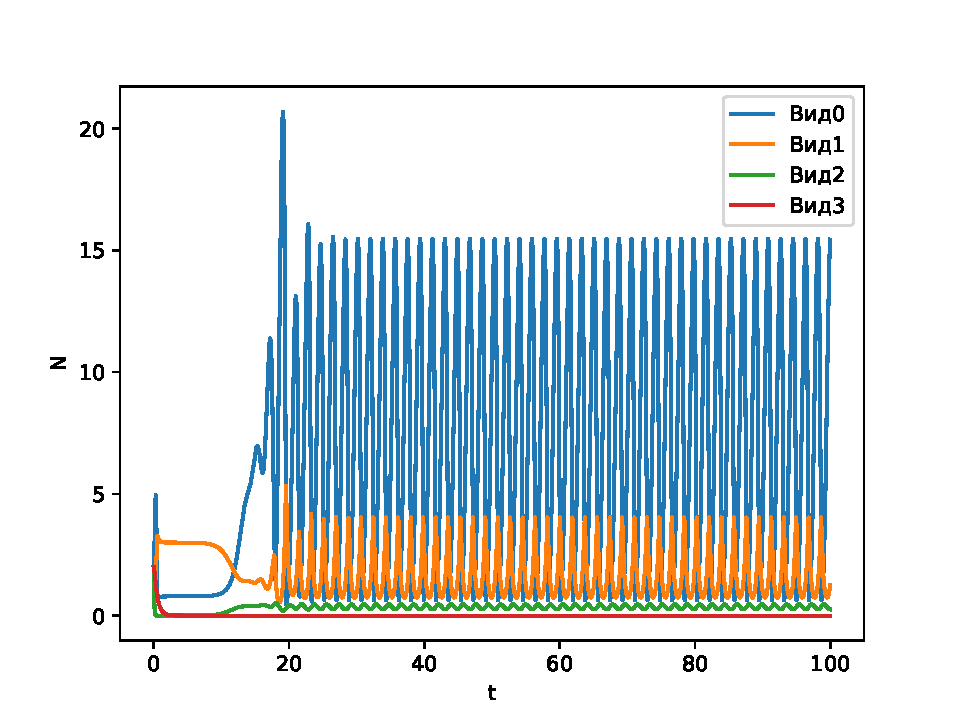
\includegraphics[width=\textwidth]{pictures/exp_flow/exp2_Q40.pdf}
            \caption{\(Q = 40\)}
        \end{subfigure}
        \begin{subfigure}[t]{.3\linewidth}
            \centering
            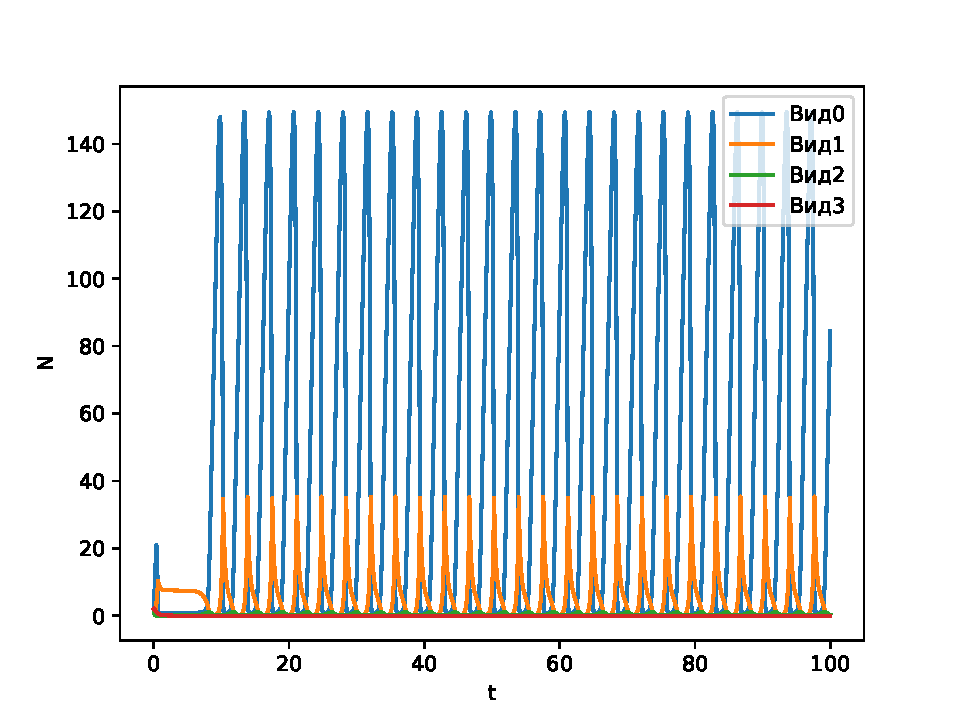
\includegraphics[width=\textwidth]{pictures/exp_flow/exp2_Q100.pdf}
            \caption{\(Q = 100\)}
        \end{subfigure}
        \begin{subfigure}[t]{.3\linewidth}
            \centering
            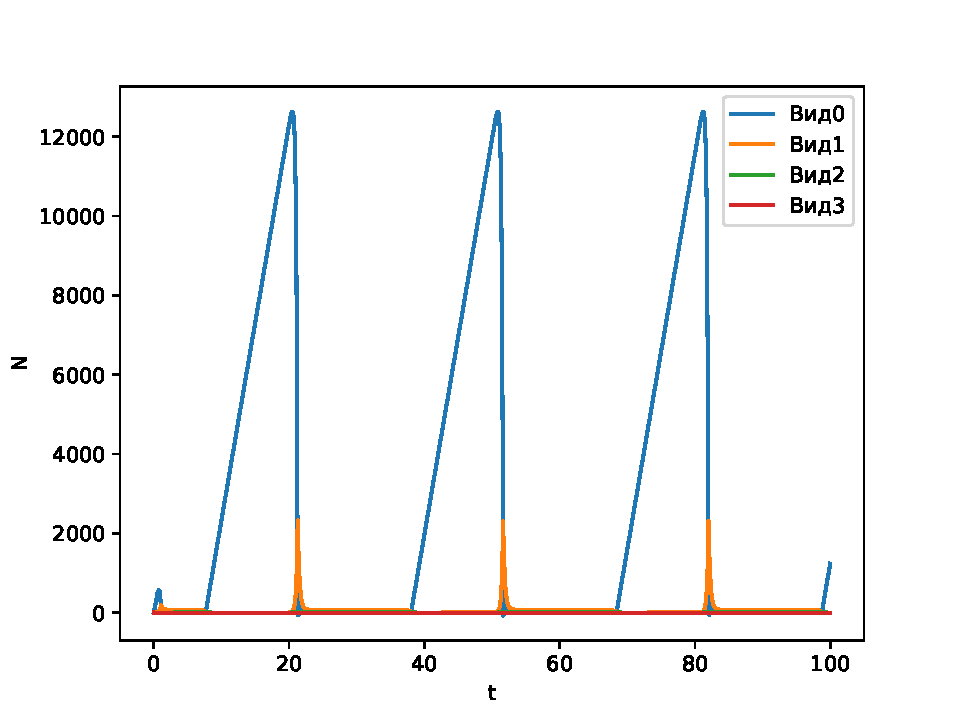
\includegraphics[width=\textwidth]{pictures/exp_flow/exp2_Q1000.pdf}
            \caption{\(Q = 1000\)}
        \end{subfigure}
    \caption{Численности видов системы.}  \label{fig:flow_exp2_q3}
    \end{figure}